\documentclass{beamer}

\usepackage[utf8]{inputenc}
\usepackage{amsfonts}
\usepackage{amsmath}
\usepackage{xcolor}
\usepackage[noend]{algpseudocode}
\usepackage{hyperref}
\usefonttheme{serif}
\usetheme{Boadilla}
\usecolortheme{seahorse}

\title[Foraging]{Biomimicry of Bacterial Foraging}
\subtitle{for Distributed Optimization and Control}
\author[Passino; Van de Kleut]{
  Kevin M. Passino\inst{1}\\
  Presented by: Alexander Van de Kleut\inst{2}
}
\institute[OST; UW]{\inst{1}
  The Ohio State University\\
  Electrical and Computer Engineering
  \and
  \inst{2}
  University of Waterloo\\
  Centre for Theoretical Neuroscience
}
\date[W20]{IEEE Control Systems Magazine, 2002}

\begin{document}

\frame{\titlepage}

\begin{frame}
\frametitle{Outline}
\tableofcontents
\end{frame}

\section{Foraging as Optimization}

\begin{frame}
\frametitle{Foraging}
\begin{itemize}
  \item<1-> \textbf{Foraging}
  \begin{itemize}
    \item<1-> searching for nutrients
    \item<1-> avoiding noxious stimuli (toxins, predators, etc)
  \end{itemize}
  \item<2-> \textbf{Social Foraging}
  \begin{itemize}
    \item<2-> increases likelihood of finding nutrients
    \item<2-> better detection and protection from noxious stimuli
  \end{itemize}
\end{itemize}
\end{frame}

\begin{frame}
\frametitle{Foraging as Optimization}
\textbf{How can we view foraging as an Optimization Process?}
\begin{itemize}
  \item<1-> We have some parameters $\theta$ and a loss function $J(\theta)$ that we want to minimize
  \item<2-> $\theta$ can represent the position of an organism in its environment
  \item<3-> $J$ can represent the concentration of nutrients and noxious stimuli
  \begin{itemize}
    \item<3-> smaller values of $J$ = more nutrients, less noxious stimuli
    \item<3-> higher values of $J$ = more noxious stimuli, less nutrients
  \end{itemize}
  \item<4-> Minimizing $J$ = foraging
\end{itemize}
\end{frame}

\section{Building the Algorithm}
\begin{frame}
\frametitle{\textit{E. coli} as a model organism}
\begin{itemize}
  \item<1-> Want foraging algorithm to be grounded in biology
  \item<2-> Model organism
  \begin{itemize}
    \item<2-> Highly studied
    \item<2-> Well-characterized foraging behaviour
  \end{itemize}
  \item<3-> Social organism
  \begin{itemize}
    \item<3-> Secretes signals to attract others nearby
    \item<3-> Encourages ``swarming'' or ``clumping''
  \end{itemize}
\end{itemize}
\end{frame}

\begin{frame}
\frametitle{\textit{E. coli} Locomotion}
\begin{itemize}
  \item<1-> Swims using left-handed helical flagella (``propellers'')
  \begin{itemize}
    \item<2-> \textbf{Tumble}: flagella all rotate clockwise $\to$ pull on cell in all directions $\to$ random movement
    \item<3-> \textbf{Run}: flagella all rotate counterclockwise $\to$ flagella form a bundle $\to$ push on cell in one direction $\to$ directed movement
  \end{itemize}
\end{itemize}
\begin{center}
\includegraphics<1->[scale=0.2]{assets/ecoli}
\end{center}
\end{frame}

\begin{frame}
\frametitle{\textit{E. coli} Foraging}
\begin{itemize}
  \item<1-> If during a tumble \textit{E. coli} swims down a nutrient concentration gradient:
  \begin{itemize}
    \item<1-> Increases probability of entering a run
    \item<1-> Continues moving down concentration gradient towards even more nutrients
  \end{itemize}
  \item<2-> Otherwise:
  \begin{itemize}
    \item<2-> Continues tumble
    \item<2-> Moves randomly to search for nutrient gradients to exploit
  \end{itemize}
  \item<3-> Call a tumble followed by a run a ``chemotaxis step''
\end{itemize}
\end{frame}

\begin{frame}
\frametitle{Algorithm for a Single Bacterium}
\begin{algorithmic}[1]
\For {$j \gets 1 \dots N_c $}:
  \State $J_\text{last} \gets J(\theta)$
  \State $\phi \sim S^p$
  \State $\theta \gets \theta + c \phi$
  \While {$J(\theta) < J_\text{last}$}:
    \State $J_\text{last} \gets J(\theta)$
    \State $\theta \gets \theta + c \phi$
  \EndWhile
\EndFor
\end{algorithmic}
\begin{itemize}
  \item $\theta$: $p$-dimensional vector (randomly initialized)
  \item $N_c$: number of chemotaxis steps
  \item $\phi \sim S^p$: a random $p$-dimensional unit vector
  \item $c$: a step-size
\end{itemize}
\end{frame}

\begin{frame}
\frametitle{Loss Function to Optimize}
\begin{center}
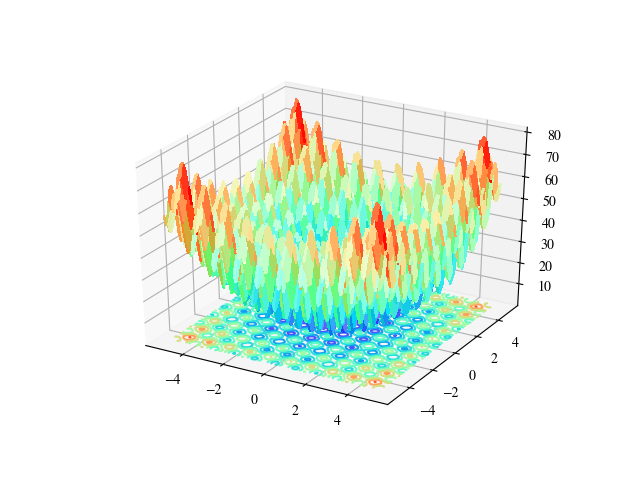
\includegraphics[scale=0.5]{assets/rastrigin}
$$J(\theta) = An + \sum_{i=1}^n \left( x_i^2 - A \cos(2 \pi x_i) \right)$$
\end{center}
\end{frame}

\begin{frame}
\frametitle{Results of Single Bacterium}
\begin{columns}[T]
  \column{0.5\textwidth}
    \begin{center}
      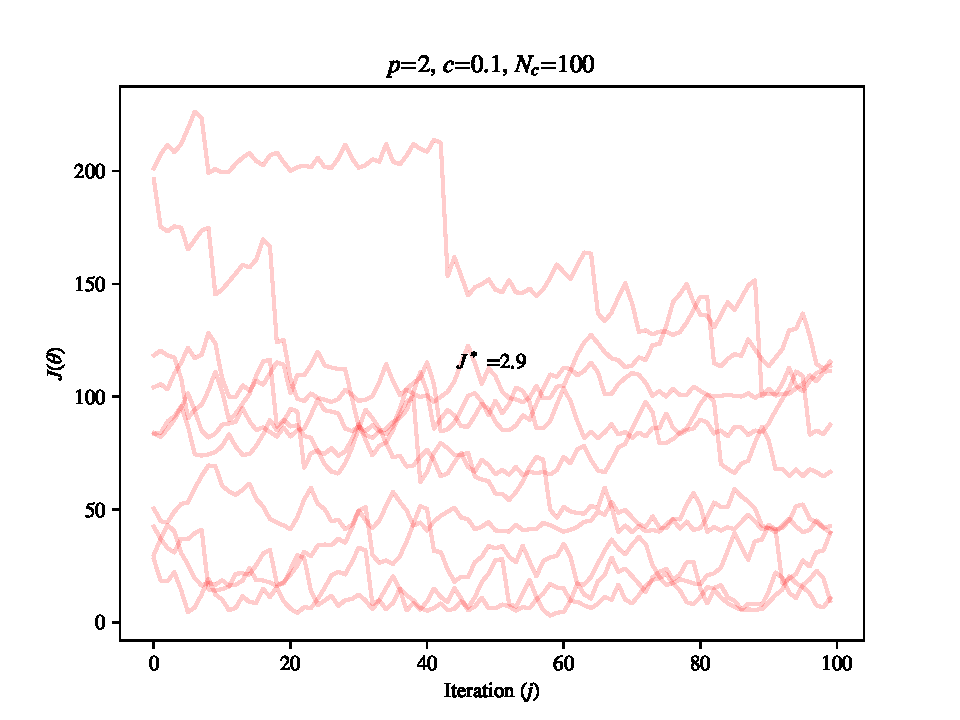
\includegraphics[scale=0.35]{assets/rastrigin_J}
    \end{center}
  \column{0.5\textwidth}
  \begin{center}
    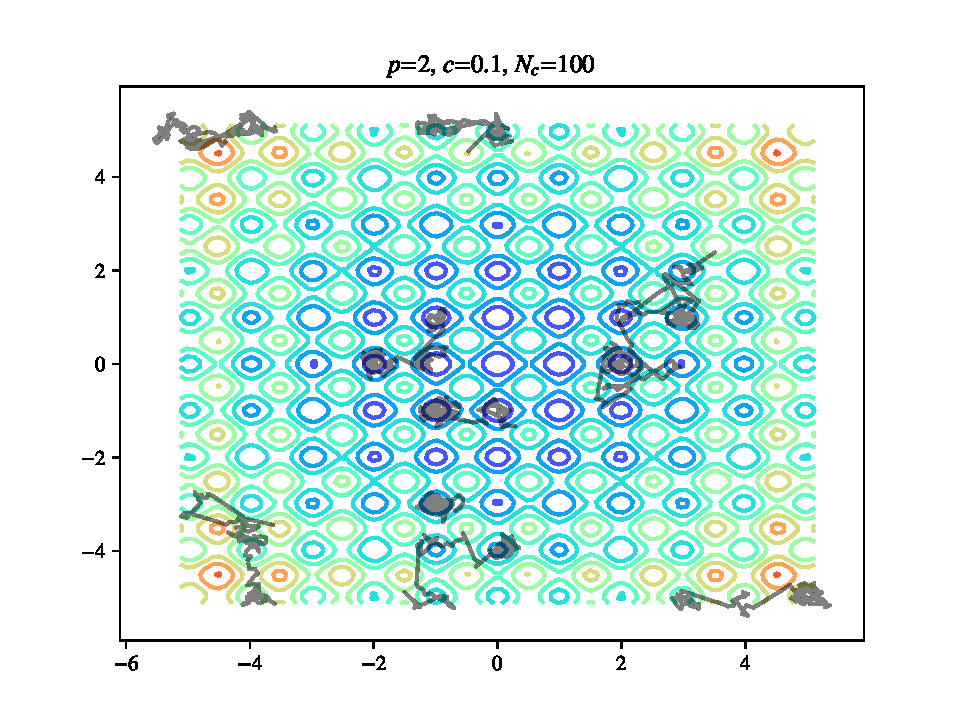
\includegraphics[scale=0.35]{assets/rastrigin_theta}
  \end{center}
\end{columns}
\end{frame}

\begin{frame}
\frametitle{$J_{cc}$ and swarming behaviour}
\begin{itemize}
  \item \textit{E. coli} do social foraging
  \item Secrete a substance to indicate to attract nearby \textit{E. coli} and encourage swarming
  \item Also want to avoid crowding
  \item Use sum of two Gaussian functions to model this
\end{itemize}
\end{frame}

\begin{frame}
\frametitle{$J_{cc}$ and swarming behaviour}
\begin{center}
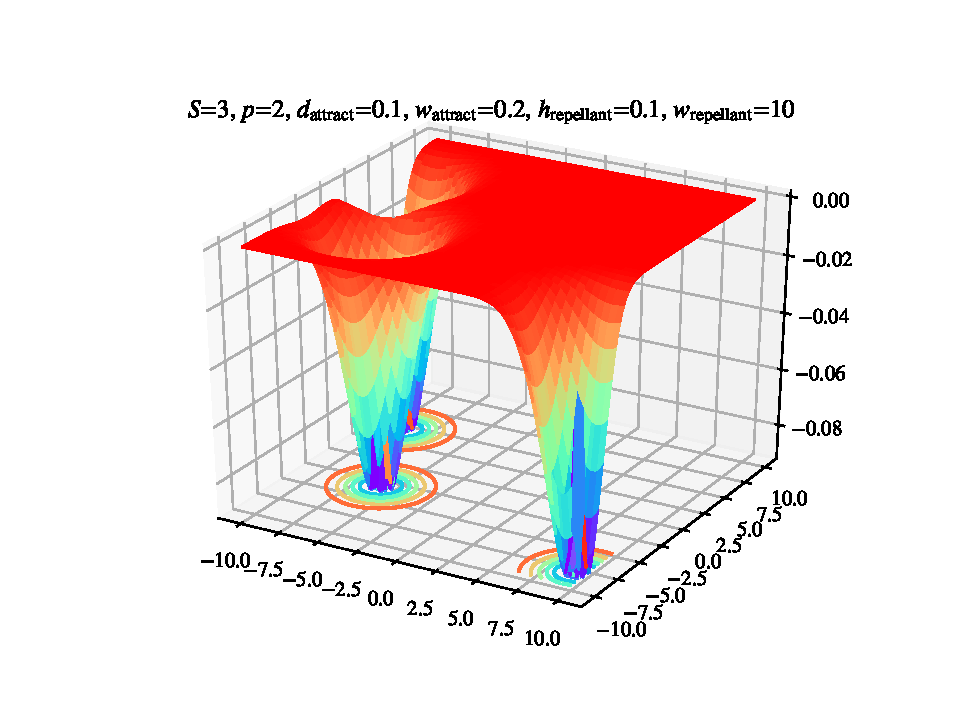
\includegraphics[scale=0.35]{assets/swarming}
\begin{align*}
J_{cc}(\theta) = \sum_{i=1}^S &-d_\text{attract} \exp \left( -w_\text{attract} (\theta - \theta_i)^T (\theta - \theta_i) \right) \\ &+ h_\text{repellant} \exp \left( -w_\text{repellant} (\theta - \theta_i)^T (\theta - \theta_i) \right)
\end{align*}
\end{center}
\end{frame}

\begin{frame}
\frametitle{Algorithm for a Colony}
\begin{algorithmic}[1]
\For {\textcolor{gray}{$j \gets 1 \dots N_c $}}:
  \For {$i \gets 1 \dots S$}:
    \State \textcolor{gray}{$J_\text{last} \gets J(\theta_i) $} $+ J_{cc}(\theta_i)$
    \State \textcolor{gray}{$\phi \sim S^p$}
    \State \textcolor{gray}{$\theta_i \gets \theta_i + c_i \phi$}
    \While {\textcolor{gray}{$J(\theta_i)$} $+ J_{cc}(\theta_i)$ \textcolor{gray}{$< J_\text{last} $}}:
      \State \textcolor{gray}{$J_\text{last} \gets J(\theta_i)$}
      \State \textcolor{gray}{$\theta_i \gets \theta_i + c_i \phi$}
    \EndWhile
  \EndFor
\EndFor
\end{algorithmic}
\begin{itemize}
  \item $S$: number of bacteria in the colony
  \item $J_{cc}$: cell-to-cell interactions
\end{itemize}
\end{frame}

\begin{frame}
\frametitle{Results of Colony with Swarming}
\begin{columns}[T]
  \column{0.5\textwidth}
    \begin{center}
      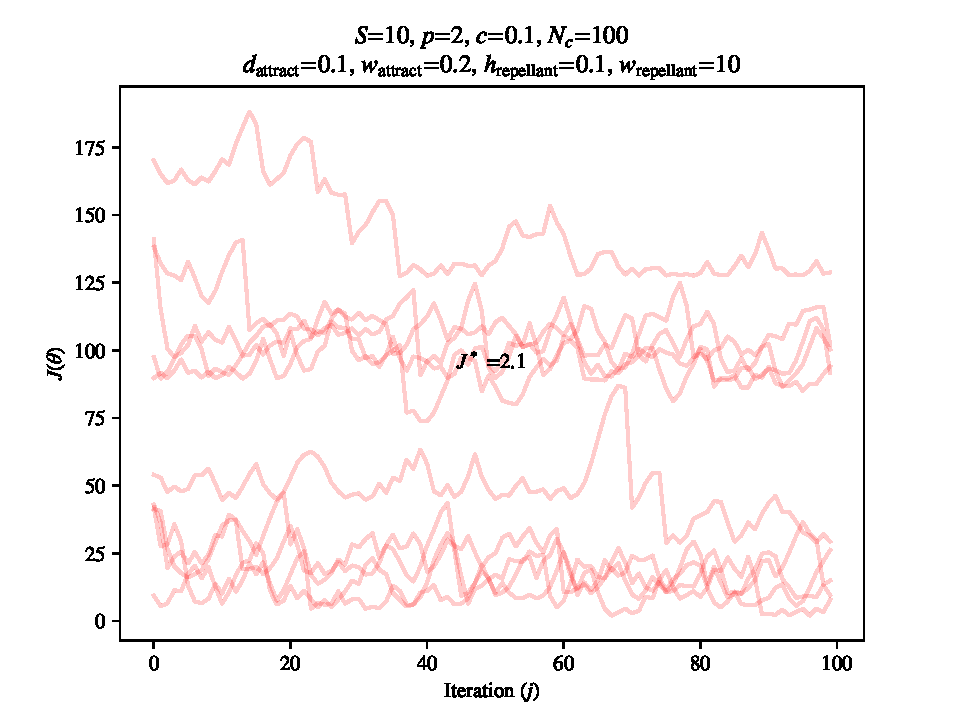
\includegraphics[scale=0.35]{assets/rastrigin_colony_J}
    \end{center}
  \column{0.5\textwidth}
  \begin{center}
    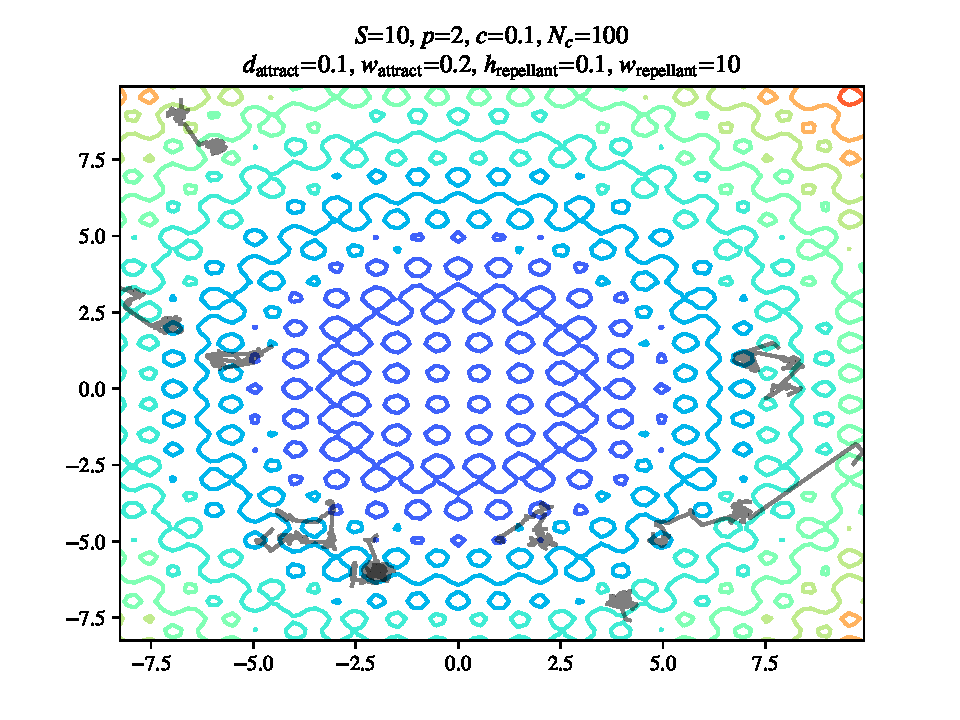
\includegraphics[scale=0.35]{assets/rastrigin_colony_theta}
  \end{center}
\end{columns}
\end{frame}

\begin{frame}
\frametitle{Results of Colony with Swarming}
\begin{columns}[T]
  \column{0.5\textwidth}
    \begin{center}
      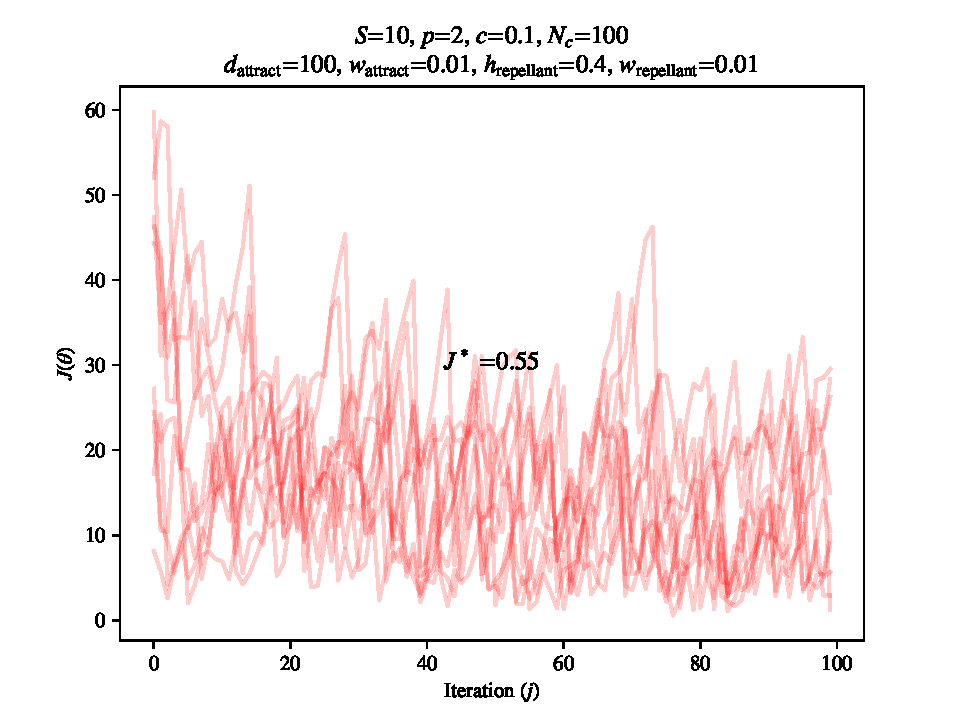
\includegraphics[scale=0.35]{assets/rastrigin_colony_tuned_J}
    \end{center}
  \column{0.5\textwidth}
  \begin{center}
    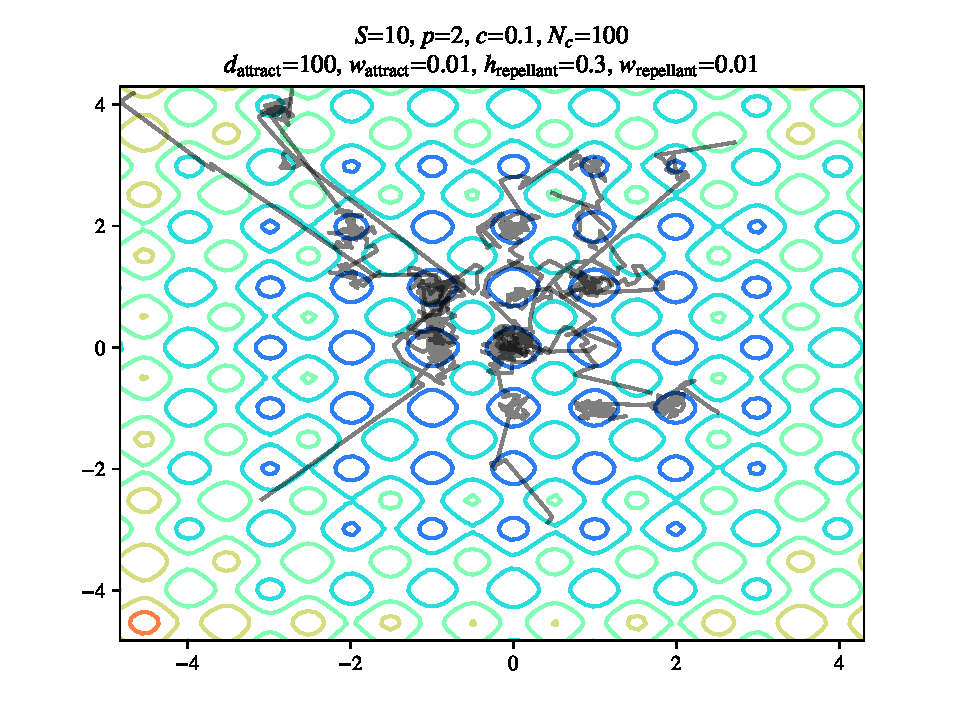
\includegraphics[scale=0.35]{assets/rastrigin_colony_tuned_theta}
  \end{center}
\end{columns}
\end{frame}

\begin{frame}
\frametitle{Comparing $J_{cc}$}
\begin{columns}[T]
  \column{0.5\textwidth}
  \begin{center}
    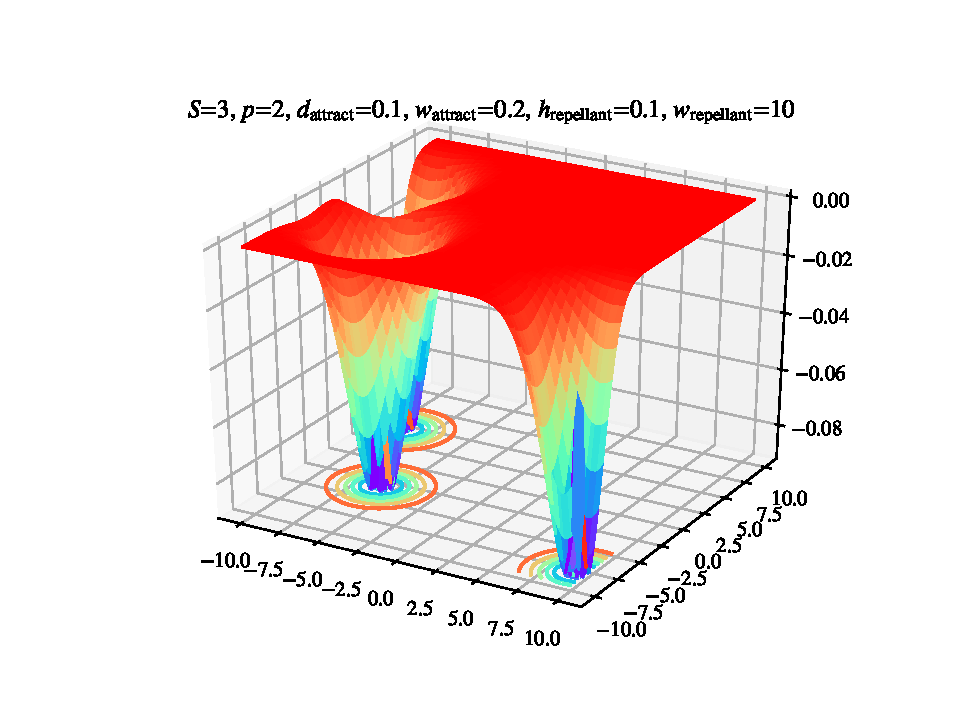
\includegraphics[scale=0.35]{assets/swarming}
  \end{center}
  \column{0.5\textwidth}
  \begin{center}
    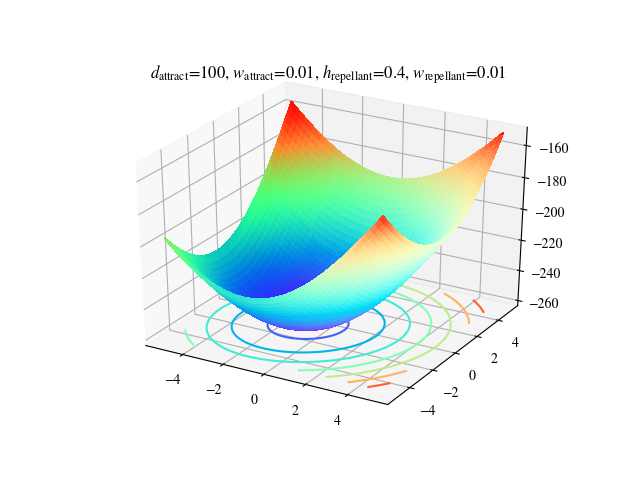
\includegraphics[scale=0.35]{assets/swarming_tuned}
  \end{center}
\end{columns}
\end{frame}

\begin{frame}
\frametitle{\textit{E. coli} reproduction}
\begin{itemize}
  \item<1-> \textit{E. coli} ``reproduce'' via binary fission, which essentially produces a clone
  \item<2-> Individuals with higher values of $J$ killed off
  \item<3-> Individuals with lower values of $J$ duplicated
  \item<4-> Idea is to encourage searching in space nearby ``best'' individuals
  \item<5-> \alert{If repellance isn't high enough then repeated iterations of evolution can concentrate colony in local minimum}
\end{itemize}
\end{frame}

\begin{frame}
\frametitle{Algorithm for a Reproducing Colony}
\begin{algorithmic}[1]
\For {$k \gets 1 \dots N_{re}$}:
  \For {\textcolor{gray}{$j \gets 1 \dots N_c $}}:
    \For {\textcolor{gray}{$i \gets 1 \dots S$}}:
      \State \textcolor{gray}{$J_\text{last} \gets J(\theta_i) + J_{cc}(\theta_i)$}
      \State \textcolor{gray}{$\phi \sim S^p$}
      \State \textcolor{gray}{$\theta_i \gets \theta_i + c_i \phi$}
      \While {\textcolor{gray}{$J(\theta_i) + J_{cc}(\theta_i) < J_\text{last} $}}:
        \State \textcolor{gray}{$J_\text{last} \gets J(\theta_i)$}
        \State \textcolor{gray}{$\theta_i \gets \theta_i + c_i \phi$}
      \EndWhile
    \EndFor
  \EndFor
  \State delete worst $S/2$ and reproduce best $S/2$
\EndFor
\end{algorithmic}
\begin{itemize}
  \item $N_{re}$: number of reproduction steps
\end{itemize}
\end{frame}

\begin{frame}
\frametitle{Results of Reproducing Colony}
\begin{columns}[T]
  \column{0.5\textwidth}
    \begin{center}
      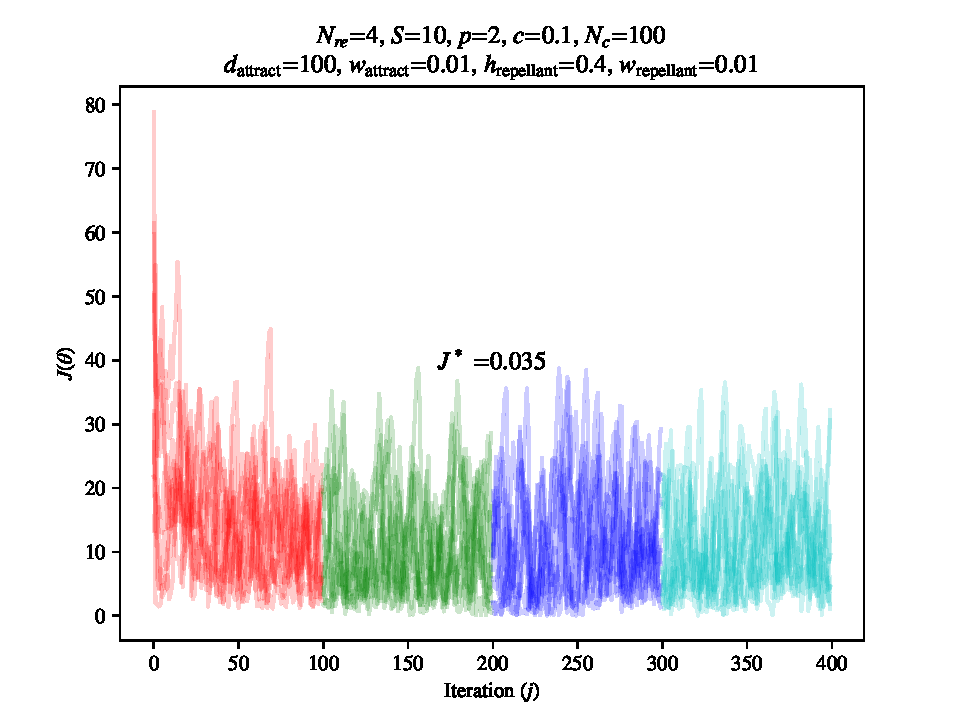
\includegraphics[scale=0.35]{assets/rastrigin_colony_re_J}
    \end{center}
  \column{0.5\textwidth}
  \begin{center}
    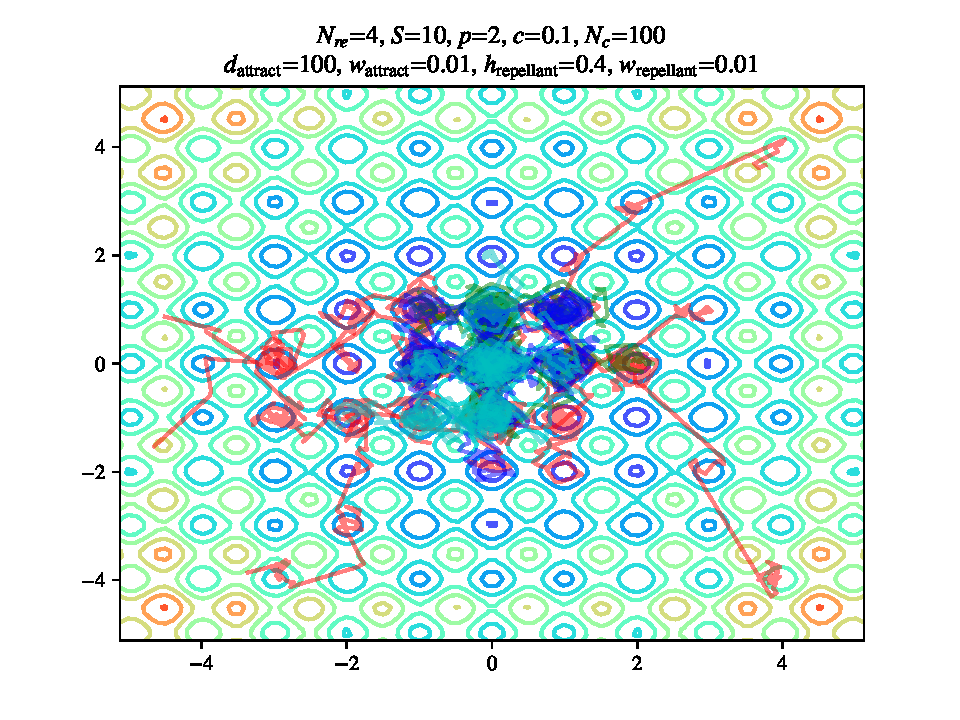
\includegraphics[scale=0.35]{assets/rastrigin_colony_re_theta}
  \end{center}
\end{columns}
\end{frame}

\begin{frame}
\frametitle{Does Reproduction Help?}
\begin{columns}[T]
  \column{0.5\textwidth}
    \begin{center}
      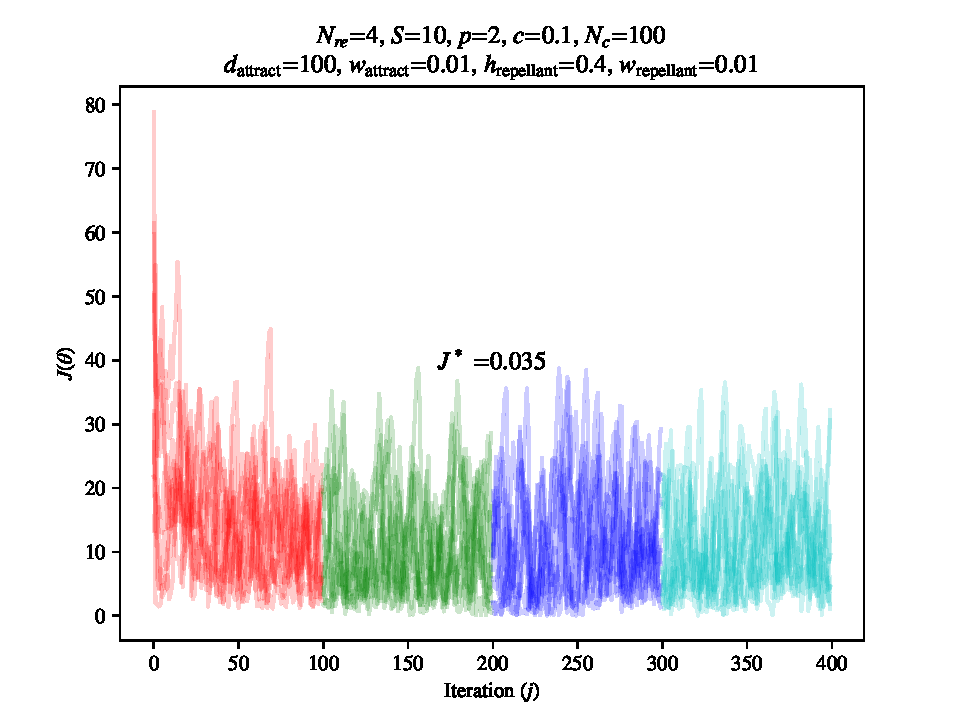
\includegraphics[scale=0.3]{assets/rastrigin_colony_re_J}
      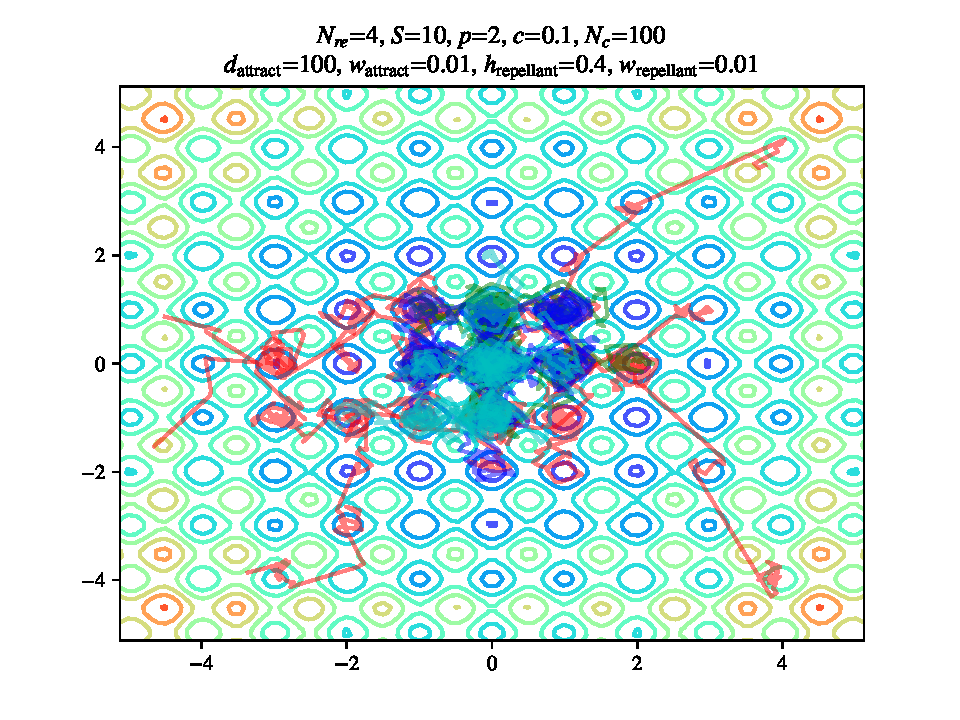
\includegraphics[scale=0.3]{assets/rastrigin_colony_re_theta}
    \end{center}
  \column{0.5\textwidth}
  \begin{center}
    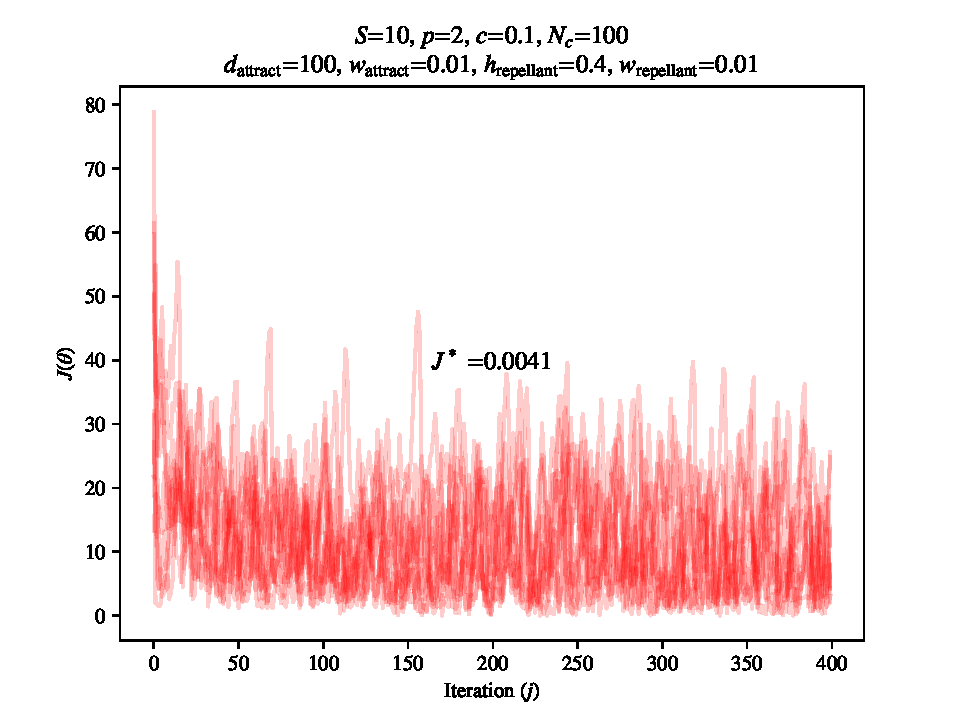
\includegraphics[scale=0.3]{assets/rastrigin_colony_400_J}
    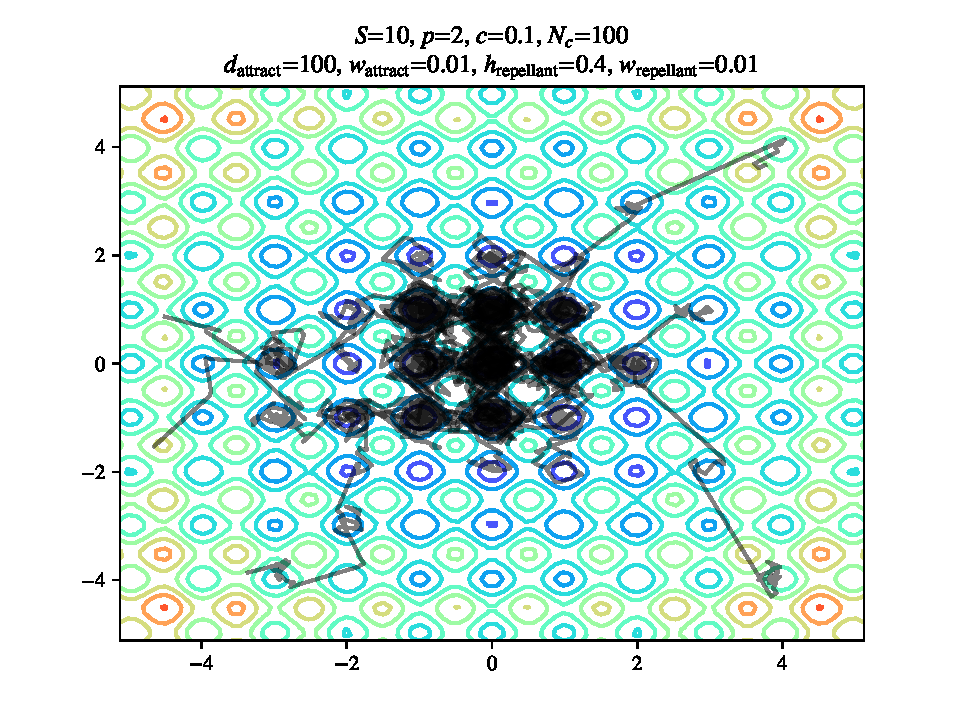
\includegraphics[scale=0.3]{assets/rastrigin_colony_400_theta}
  \end{center}
\end{columns}
\end{frame}

\begin{frame}
\frametitle{Elimination-Dispersal Events}
\begin{columns}[T]
\column{0.5\textwidth}
\begin{center}
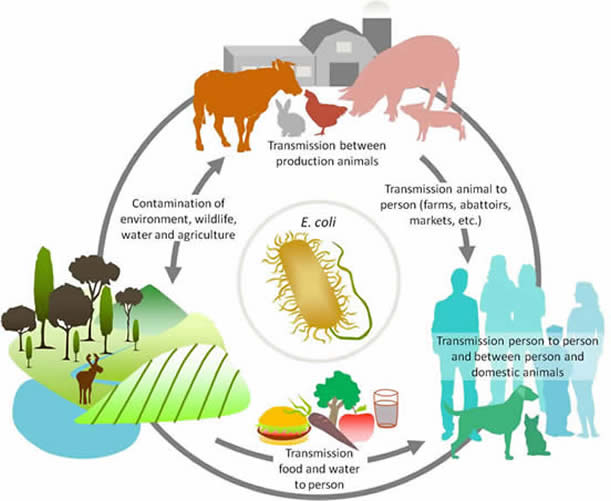
\includegraphics[scale=0.25]{assets/transmission.jpg}
\end{center}
\column{0.5\textwidth}
\begin{itemize}
  \item<1-> Over time, random events disperse populations of \textit{E. coli}

  \item<2-> May destroy chemotactic progress
  \begin{itemize}
    \item<2-> But may also bring \textit{E. coli} to good food sources
  \end{itemize}
  \item<3-> For optimization, this is a method to prevent stagnation and move out from local minima
\end{itemize}
\end{columns}
\end{frame}

\begin{frame}
\frametitle{Algorithm for a Dispersing Colony}
\begin{algorithmic}[1]
\For {$l \gets 1 \dots N_{ed}$}:
  \For {\textcolor{gray}{$k \gets 1 \dots N_{re}$}}:
    \For {\textcolor{gray}{$j \gets 1 \dots N_c $}}:
      \For {\textcolor{gray}{$i \gets 1 \dots S$}}:
        \State \textcolor{gray}{$J_\text{last} \gets J(\theta_i) + J_{cc}(\theta_i)$}
        \State \textcolor{gray}{$\phi \sim S^p$}
        \State \textcolor{gray}{$\theta_i \gets \theta_i + c_i \phi$}
        \While {\textcolor{gray}{$J(\theta_i) + J_{cc}(\theta_i) < J_\text{last} $}}:
          \State \textcolor{gray}{$J_\text{last} \gets J(\theta_i)$}
          \State \textcolor{gray}{$\theta_i \gets \theta_i + c_i \phi$}
        \EndWhile
      \EndFor
    \EndFor
    \State \textcolor{gray}{delete worst $S/2$ and reproduce best $S/2$}
  \EndFor
  \For {$i \gets 1 \dots S$}:
    \If {$\epsilon \sim \mathcal{U}(0, 1) < p_{ed}$}:
      \State $\theta_i \sim d^0(\theta)$
    \EndIf
  \EndFor
\EndFor
\end{algorithmic}
\begin{itemize}
  \item $N_{ed}$: number of elimination-dispersal events
  \item $p_{ed}$: probabilty of a single elimination-dispersal event
\end{itemize}
\end{frame}

\begin{frame}
\frametitle{Results of Elimination-Dispersal}
\begin{columns}[T]
  \column{0.5\textwidth}
    \begin{center}
      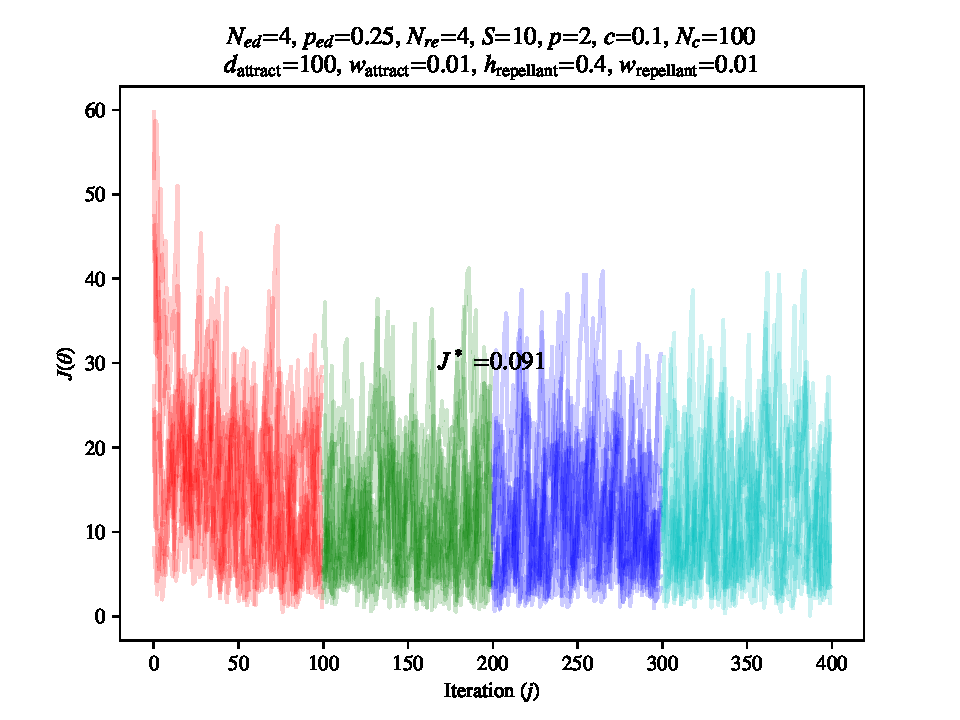
\includegraphics[scale=0.3]{assets/rastrigin_colony_ed_0_J}
      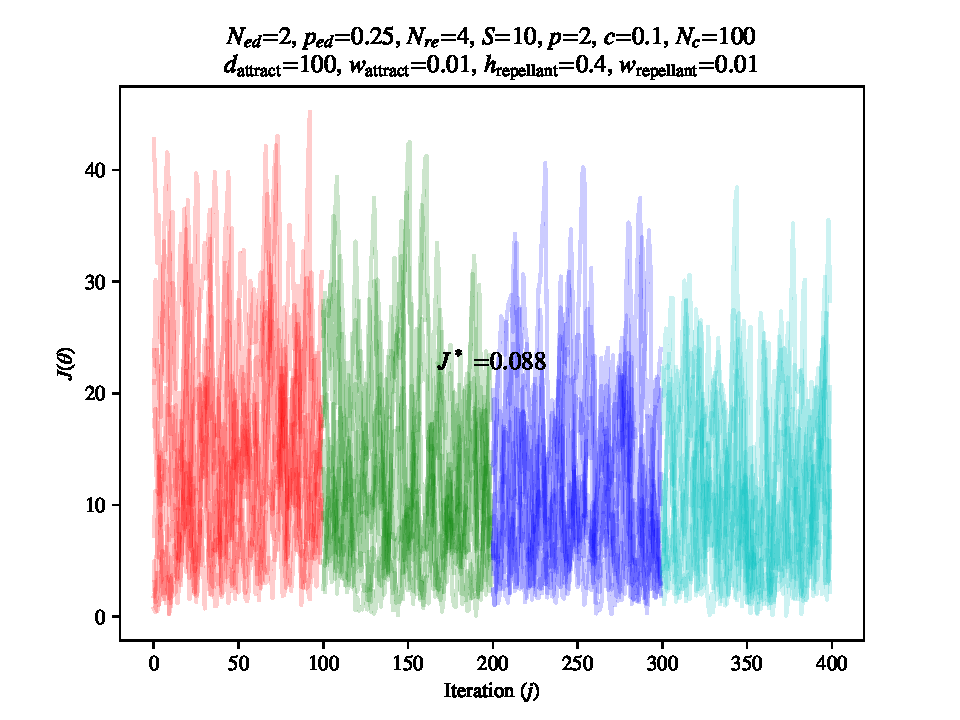
\includegraphics[scale=0.3]{assets/rastrigin_colony_ed_1_J}
    \end{center}
  \column{0.5\textwidth}
  \begin{center}
    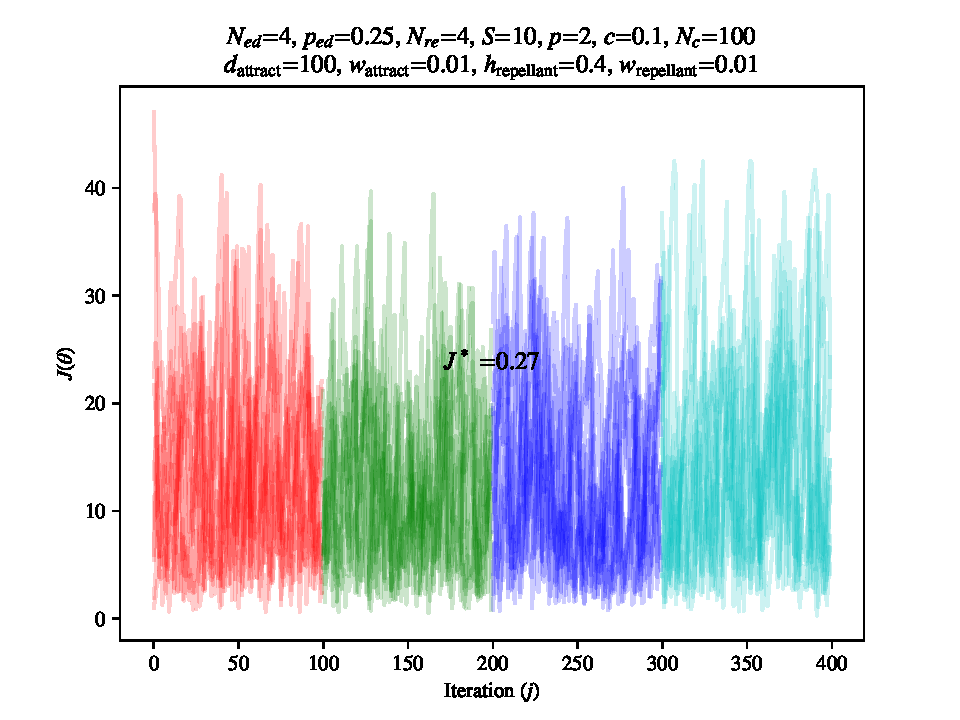
\includegraphics[scale=0.3]{assets/rastrigin_colony_ed_2_J}
    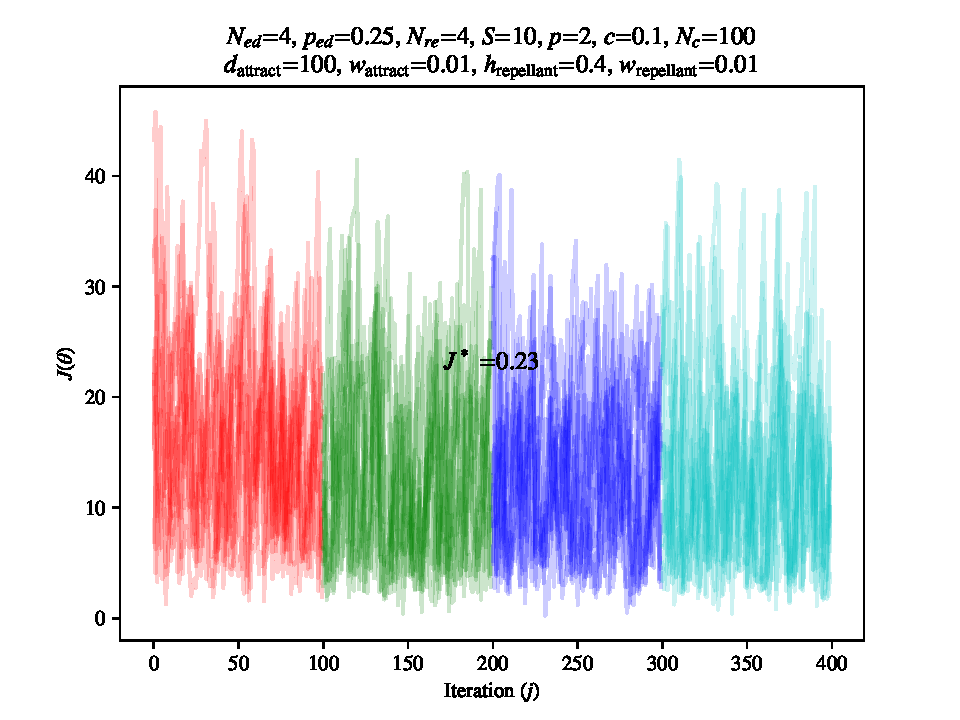
\includegraphics[scale=0.3]{assets/rastrigin_colony_ed_3_J}
  \end{center}
\end{columns}
\end{frame}

\section{Discussion}

\begin{frame}
\frametitle{Is this a good optimization algorithm?}
\begin{itemize}
  \item<2-> We don't know. The author doesn't compare to any existing methods.
  \item<3-> The author draws a comparison to genetic algorithms (GAs) since both are hill-climbing algorithms, but asserts that they are really different algorithms \textbf{based on their biological inspiration}
  \item<4-> The method is also suspiciously similar to partical swarm optimization
  \begin{itemize}
    \item<5-> Combines local and global information with stochastic hill-climbing algorithm
    \item<5-> The author never mentions this despite the popularity of PSOs (this paper publish 7 years later)
    \item<6-> (Ask me about the comparison I did afterwards!)
  \end{itemize}
\end{itemize}
\end{frame}

\begin{frame}
\frametitle{Is this a good optimization algorithm?}
\begin{itemize}
  \item<1-> However, this algorithm is \textbf{gradient-free}
  \begin{itemize}
    \item<2-> We can minimize functions that we may not have access to the gradient for (or it may not exist)
    \item<2-> For example tuning hyperparameters
  \end{itemize}
  \item<3-> It can also explore the search space beyond the initial distribution $d^0(\theta)$ in case we do not know where the optimal value $\theta^*$ lies
\end{itemize}
\end{frame}

\begin{frame}
\frametitle{Is this a good model of \textit{E. coli}?}
\begin{itemize}
  \item<2-> We don't know. The author doesn't compare to any ecological data.
  \item<3-> Some important limitations from the author:
  \begin{itemize}
    \item<4-> Ignores biology in favour of chemotactic hill-climbing and swarming
    \item<5-> Assumes organisms do not modify the nutrient surface
    \item<6-> Assumes a constant population size
  \end{itemize}
\end{itemize}
\end{frame}

\begin{frame}
\frametitle{Is this a good model of \textit{E. coli}?}
\begin{center}
\includegraphics<1->[scale=0.3]{assets/yikes}
\end{center}
\begin{itemize}
  \item<1-> It is not clear if the goal is create a simulation of \textit{E. coli} foraging behaviour or to create another biologically-inspired optimization algorithm
\end{itemize}
\end{frame}

\begin{frame}
\frametitle{Discussion}
\begin{center}
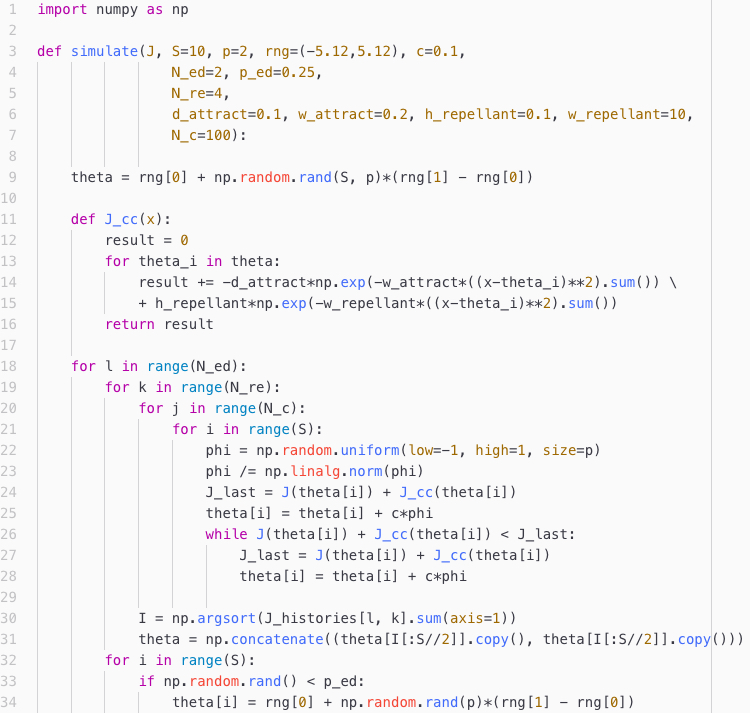
\includegraphics[scale=0.25]{assets/code}
\href{github.com/avandekleut/bacterial-foraging}{https://github.com/avandekleut/bacterial-foraging/}
\end{center}
\end{frame}

\begin{frame}
\frametitle{Methods compared}
\begin{center}
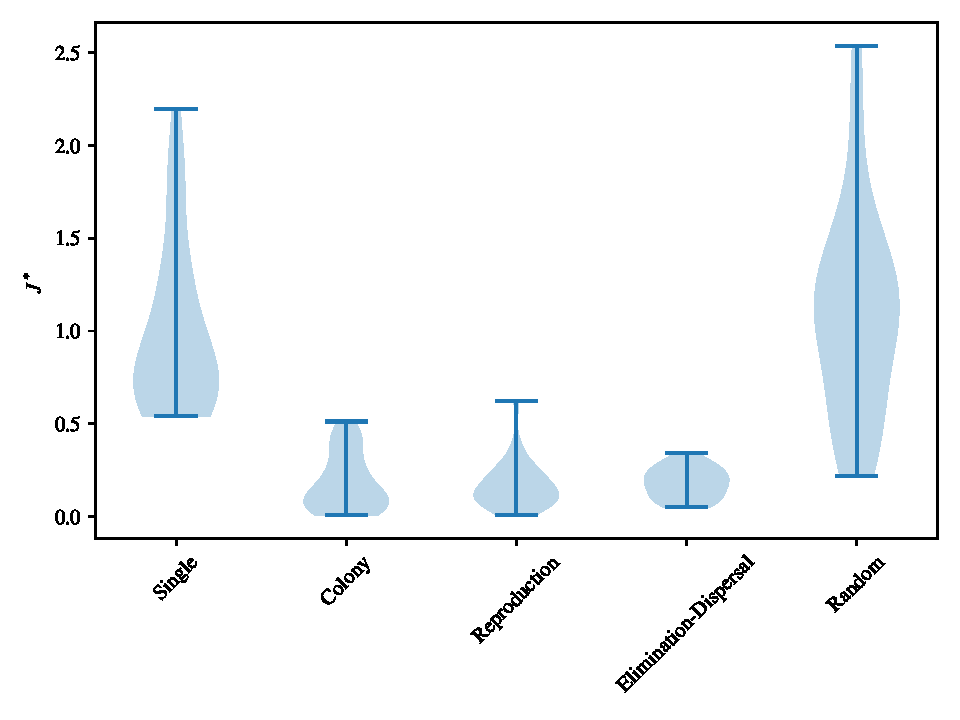
\includegraphics[scale=0.5]{assets/compared}
\end{center}
\end{frame}

\begin{frame}
\frametitle{Comparison to PSO}
\begin{itemize}
  \item Bacterial foraging method:
  \begin{itemize}
    \item   At least $N_{ed} \times N_{re} \times S \times N_c$ values of $\theta$ seen
  \end{itemize}
  \item PSO: $N \times \text{iter}$ values of $\theta$ seen
  \begin{itemize}
    \item PSO strongest with large $N$, so presume $\text{iter} \equiv N_c$
    \item Then $N = N_{ed} \times N_{re} \times S$
  \end{itemize}
\end{itemize}
\end{frame}

\begin{frame}
\frametitle{Comparison to PSO}
\begin{columns}[T]
  \column{0.5\textwidth}
    \begin{center}
      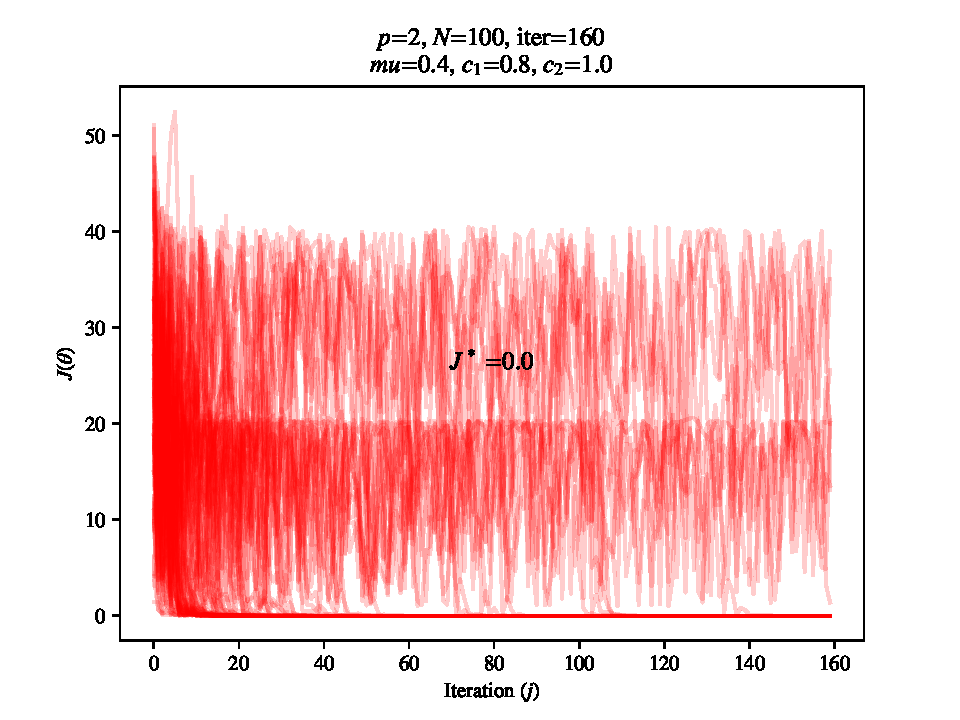
\includegraphics[scale=0.3]{assets/pso_J}
      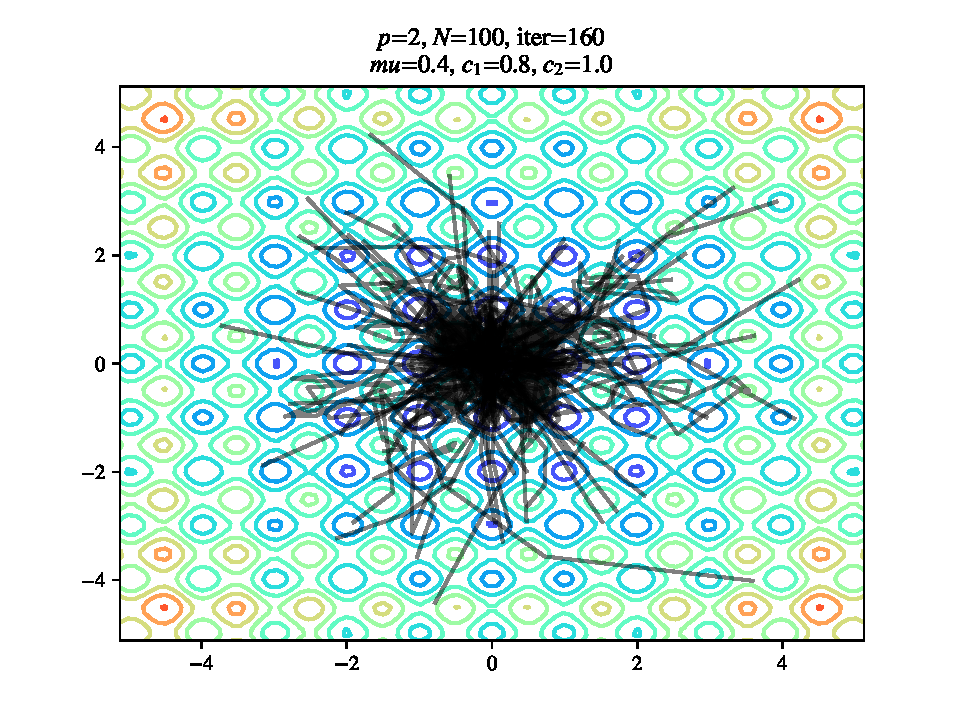
\includegraphics[scale=0.3]{assets/pso_theta}
    \end{center}
  \column{0.5\textwidth}
  \begin{center}
    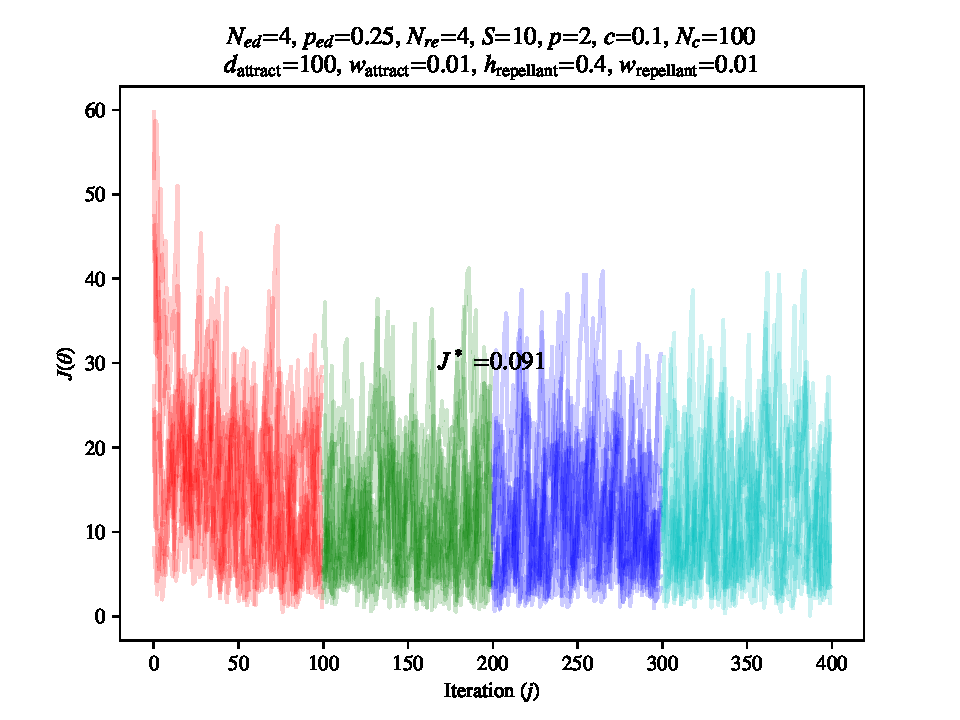
\includegraphics[scale=0.3]{assets/rastrigin_colony_ed_0_J}
    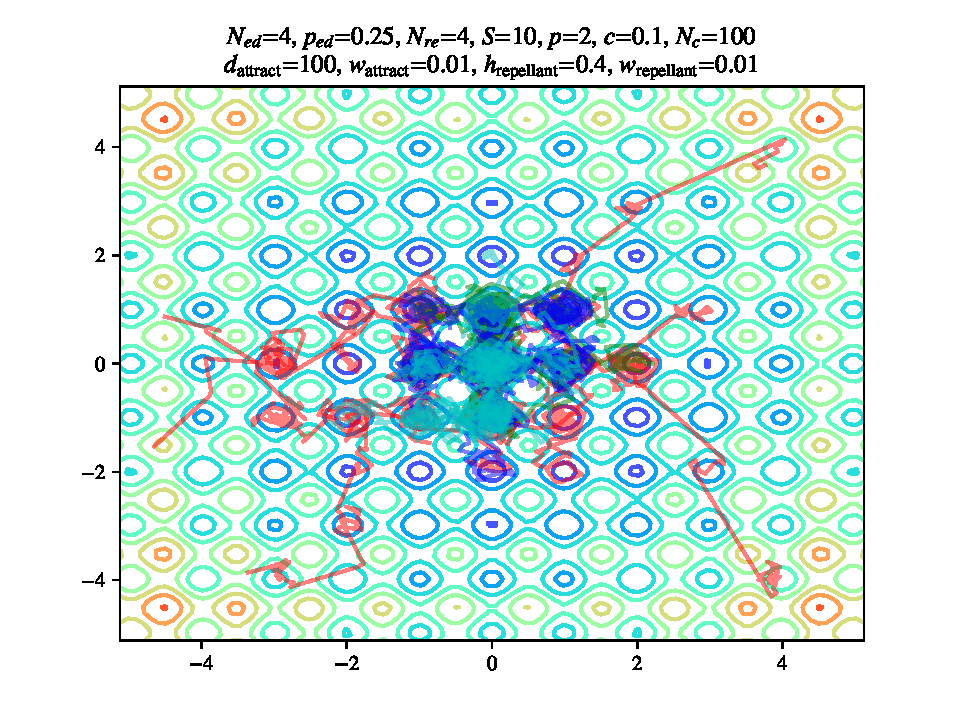
\includegraphics[scale=0.3]{assets/rastrigin_colony_ed_0_theta}
  \end{center}
\end{columns}
\end{frame}

\end{document}
